\Transcb{yellow}{blue}{Hunting for Cosmic Neutrino sources}
\twocolumn
\begin{center}
\colorbox{yellow}{Neutrino production mechanism}\\
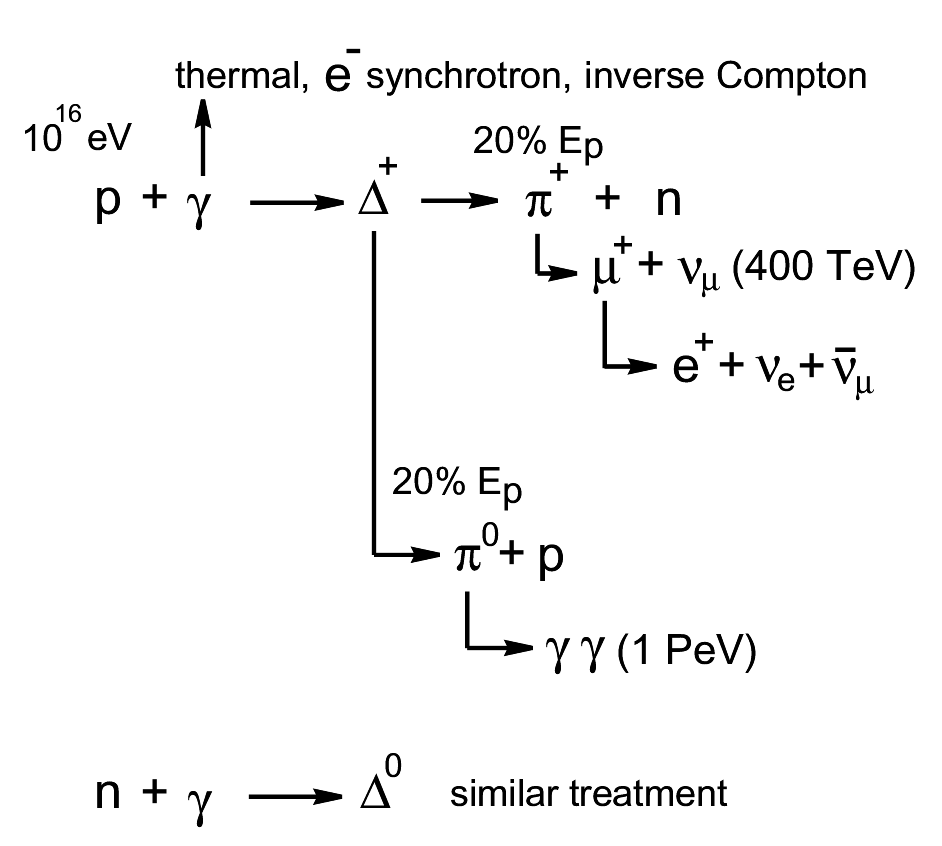
\includegraphics[keepaspectratio,width=13cm]{grb-engine2}
\end{center}
%
\begin{itemize}
\item $\Delta$ prod. threshold~: $E_{\gamma} \ge 10$ eV\\
      (UV photons)
\end{itemize}

\newpage
%
\begin{itemize}
\item {\red Waxmann-Bahcall} {\large [PRL 78 (1997) 2292]}
\item[] High-E $p$ diffuse out of the shocks
\item[] Observed CR $\rightarrow$ lower limit on $p$ flux 
\item[] {\blue Fraction of $p$ used for $\nu$ production ?}
\item {\red M. Ahlers et al.} {\large [APP 35 (2011) 87]}
\item[] Protons trapped, neutrons escape
\item[] CR observations provide the $n$ flux
\item[] {\blue Direct relation CR $\leftrightarrow \nu$ flux}
\item {\red Generic $\nu$ spectrum} {\large [JCAP 0903 (2009) 020]}
\item[] 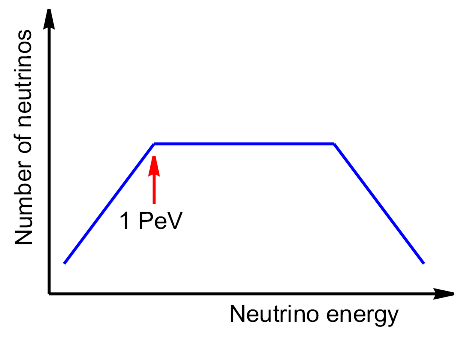
\includegraphics[keepaspectratio,height=6cm]{wb-spectrum}
\end{itemize}

\Tr
\onecolumn
\begin{center}
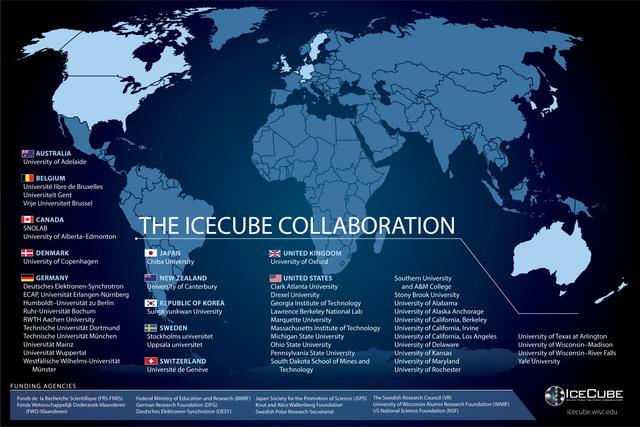
\includegraphics[keepaspectratio,height=15cm]{icecube-collab2}
\end{center}

\Tr
\onecolumn
\begin{center}
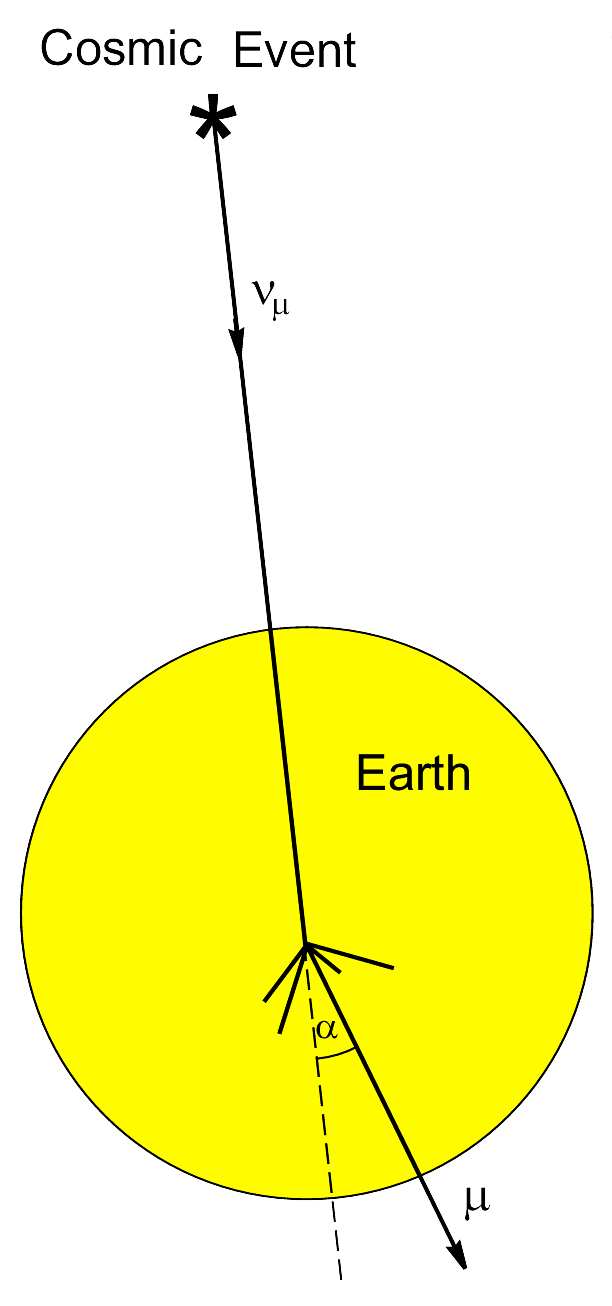
\includegraphics[keepaspectratio,height=14cm]{earth-shield} $\quad$
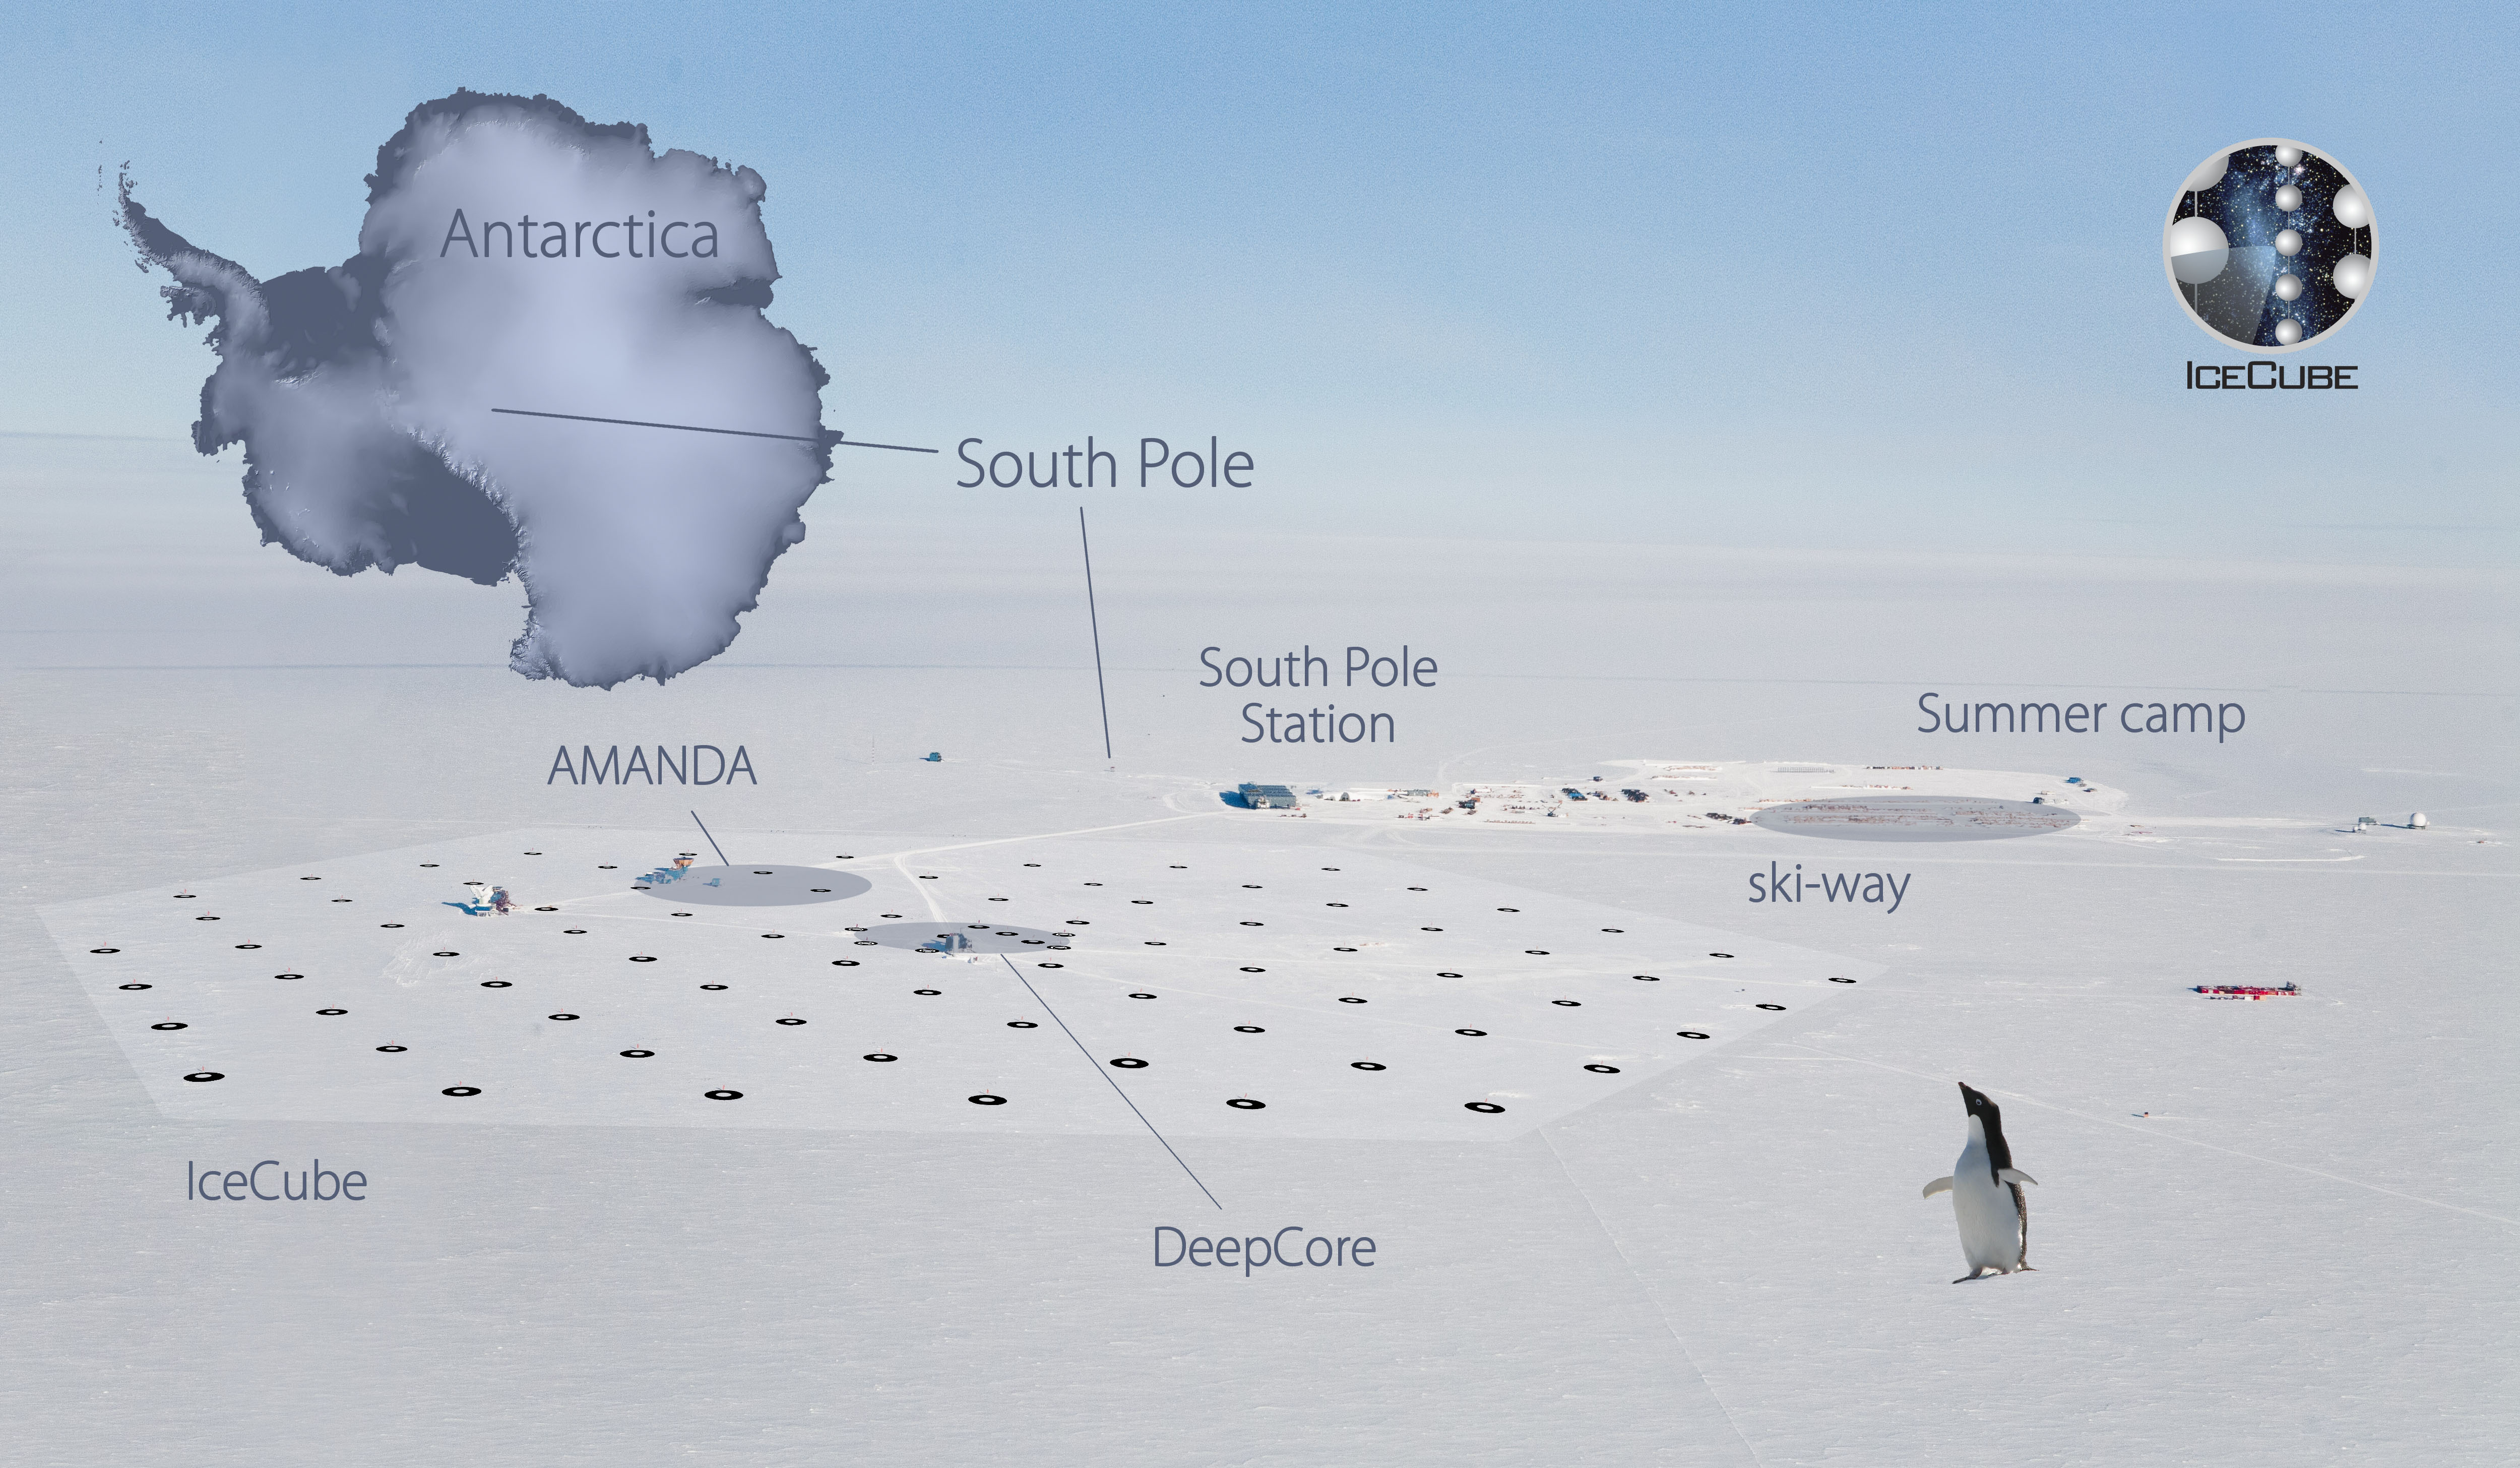
\includegraphics[keepaspectratio,width=18cm]{pole-view}
\end{center}

\Tr
\onecolumn
\begin{center}
{\blue The IceCube Neutrino Observatory at the South Pole}\\
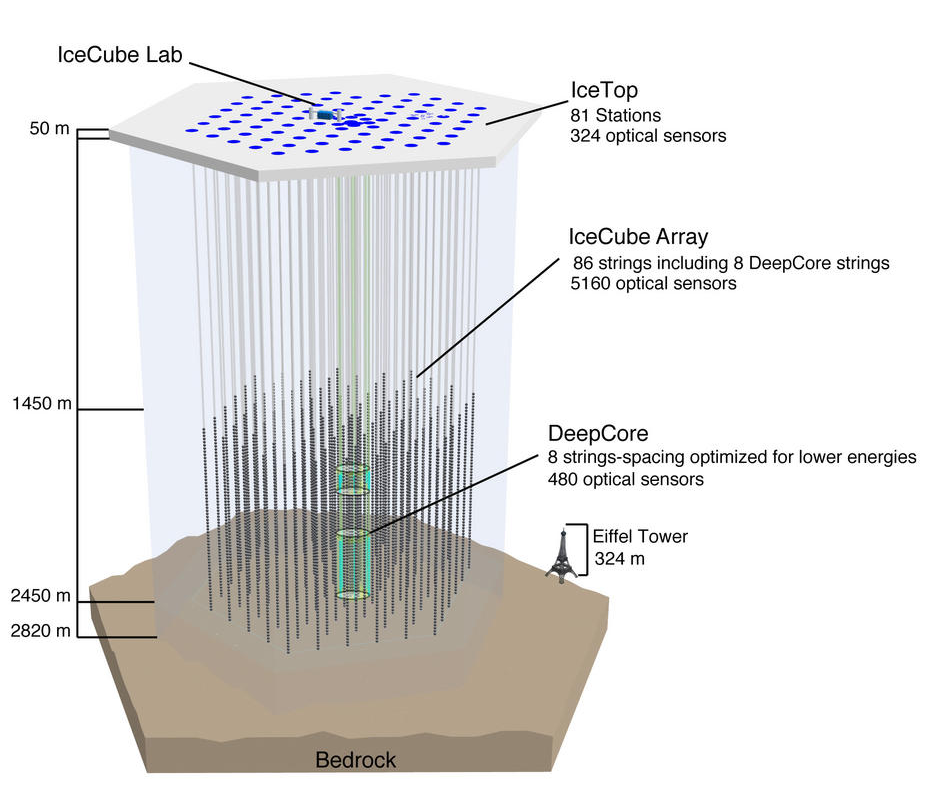
\includegraphics[keepaspectratio,height=14cm]{ic86-dc}\\
86 strings, 5160 optical sensors, instrumented volume $\sim 1~\rm{km}^{3}$
\end{center}

\Tr
\onecolumn
\begin{center}
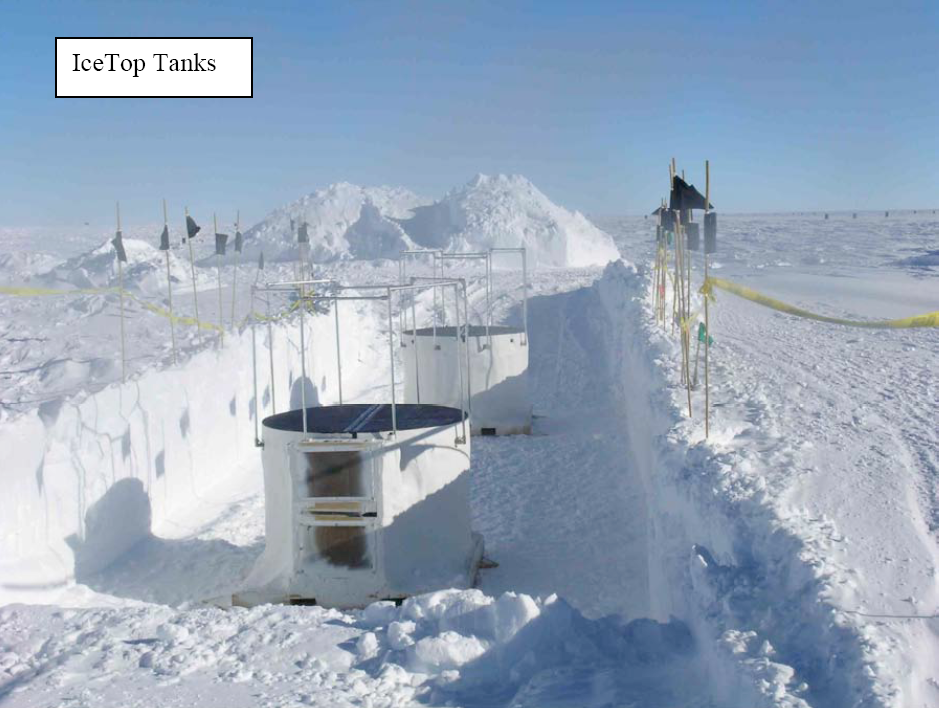
\includegraphics[keepaspectratio,height=14.5cm]{icetop-snow}
\end{center}

\Tr
\onecolumn
\begin{center}
{\blue The IceTop detection principle}\\[5mm] 
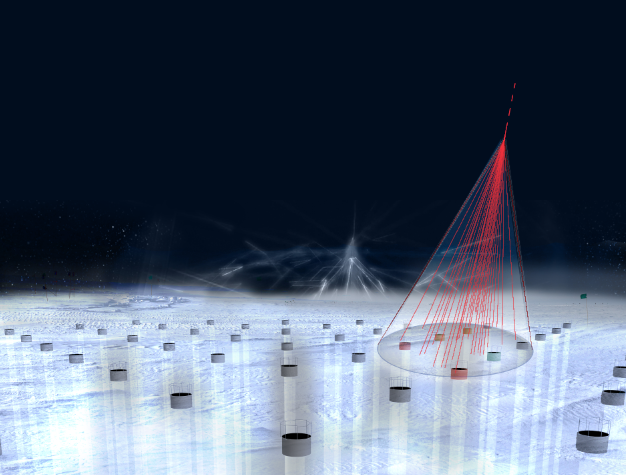
\includegraphics[keepaspectratio,height=14cm]{cr-shower2}
\end{center}

\Tr
\onecolumn
\begin{center}
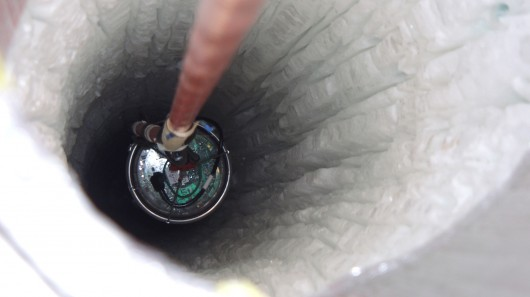
\includegraphics[keepaspectratio,height=14cm]{hole2}
\end{center}

\Tr
\twocolumn[\begin{center}{\blue The InIce detection principle}\end{center}]
\begin{center}
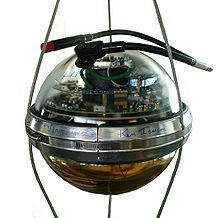
\includegraphics[keepaspectratio,height=6cm]{dom}\\[3mm]
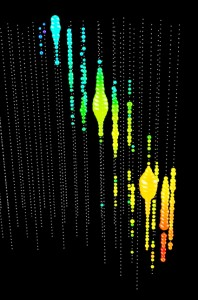
\includegraphics[keepaspectratio,height=7cm]{event}
\end{center}
%
\newpage
%
\begin{center}
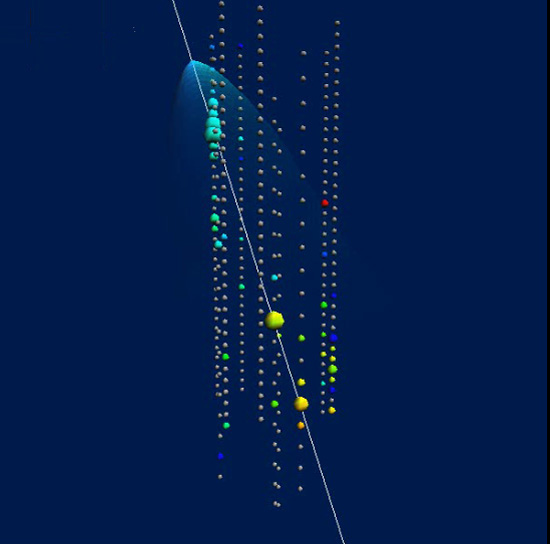
\includegraphics[keepaspectratio,width=13.5cm]{cone}
\end{center}

\Tr
\onecolumn
\begin{center}
{\red Muons from atmospheric interactions}\\[1cm]
{\blue The shadow of the Moon}\\[5mm]
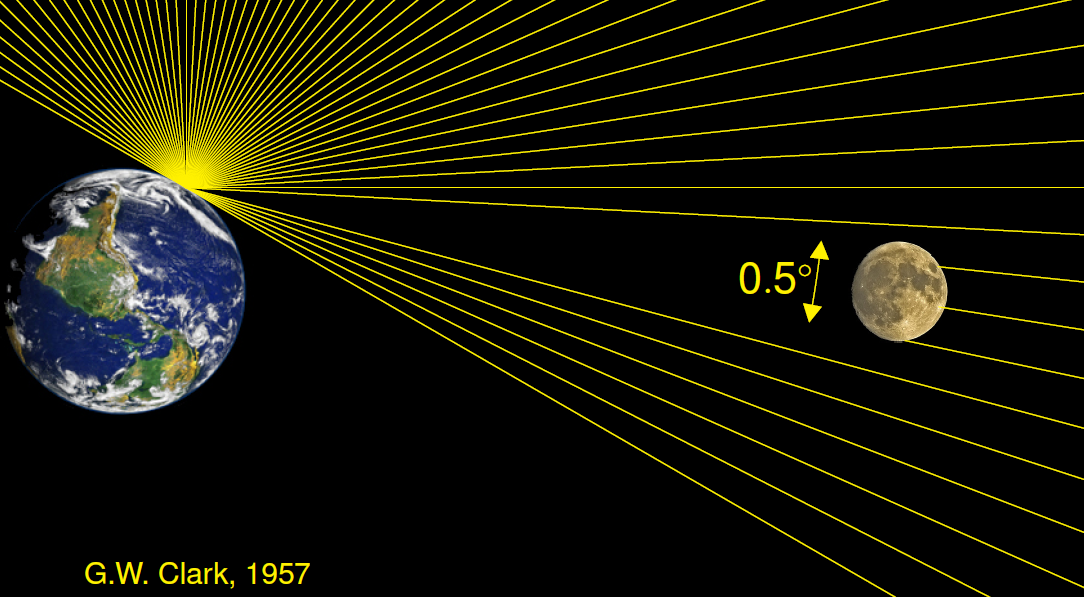
\includegraphics[keepaspectratio,height=8cm]{moon-shadow1}
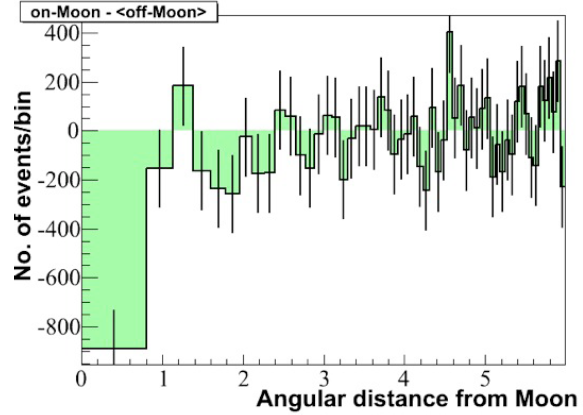
\includegraphics[keepaspectratio,height=8cm]{moon-shadow2}\\[1cm]
{\blue Angular resolution : $\sim 0.8^{\circ}$}
\end{center}

\Tr
\onecolumn
\begin{center}
{\blue IceCube 7-years skymap ($\sim$700'000 events)} {\large [ApJ 835 (2017) 151]}
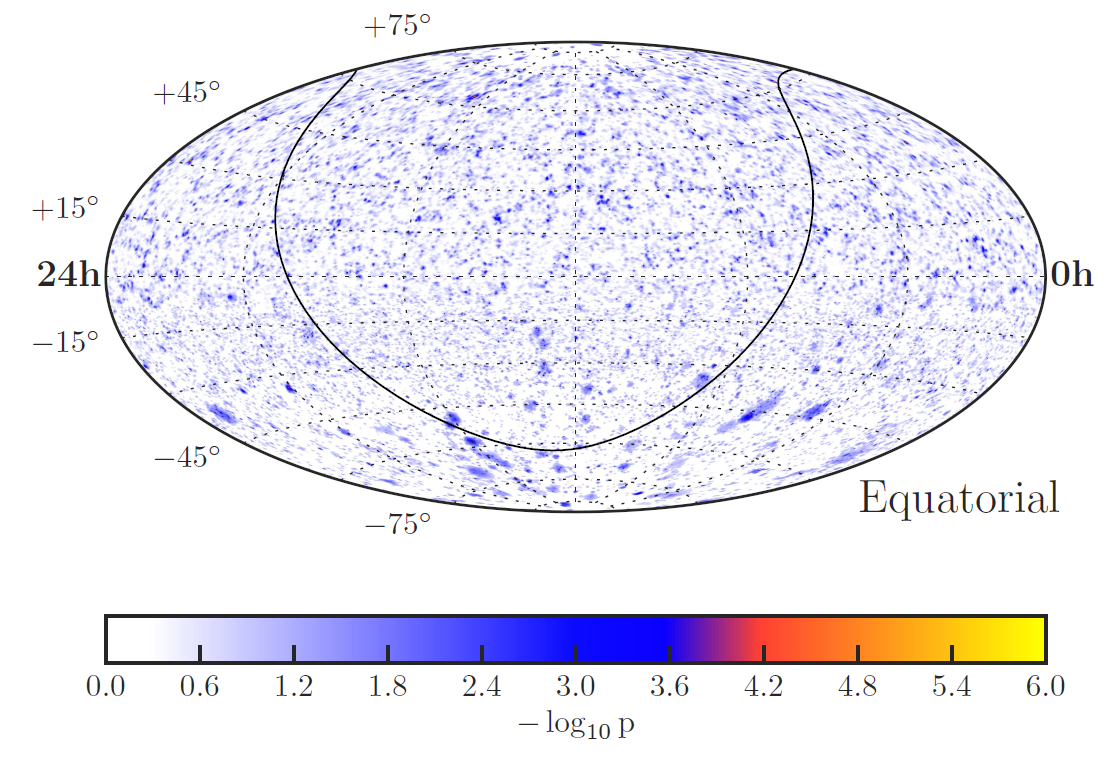
\includegraphics[keepaspectratio,height=13cm]{icecube-skymap-7years}\\
\colorbox{yellow}{No evidence for point sources (yet)}
\end{center}
